\documentclass[12pt,letterpaper,onecolumn]{article}
\usepackage[utf8]{inputenc}
\usepackage{amsmath}
\usepackage{amsfonts}
\usepackage{amssymb}
\usepackage{graphicx}
\usepackage{lipsum}  
\usepackage{placeins} % added to use float barrier
\usepackage[left=3.35cm,right=3.96cm,top=1.905cm,bottom=2.36cm]{geometry}
\usepackage{indentfirst} % indent the first paragraph after the section label

% use a times font
\usepackage{times}

% change the figure caption label from Figure: to Figure.
\usepackage{caption}
\captionsetup{labelsep = period}

% update the abstract layout
\usepackage{abstract}
\renewcommand{\absnamepos}{flushleft}
\renewcommand\abstractname{\uppercase{Abstract}}
\setlength{\absleftindent}{0mm}
\setlength{\absrightindent}{0mm}
  
% change the reference format from [1] to 1.
\makeatletter
\renewcommand\@biblabel[1]{#1.}
\makeatother

% remove space between lines in the bibliography
\let\OLDthebibliography\thebibliography
\renewcommand\thebibliography[1]{
  \OLDthebibliography{#1}
  \setlength{\parskip}{0pt}
  \setlength{\itemsep}{0pt plus 0.3ex}
}

% update the section layout
\usepackage{titlesec}  
\titleformat{\section}
  {\normalfont\bfseries\uppercase}   % The style of the section title
  {}                                 % a prefix
  {0pt}                              % How much space exists between the prefix and the title
  {}                                 % How the section is represented
\titlespacing*{\section}
{0pt}{2\baselineskip}{1\baselineskip}

% update the subsection layout
\titleformat{\subsection}
  {\normalfont\bfseries}           
  {}                               
  {0pt}                         
  {}                             
\titlespacing*{\subsection}
{0pt}{1\baselineskip}{1\baselineskip}

% update the subsubsection layout
\titleformat{\subsubsection}
  {\normalfont\uppercase}         
  {}                              
  {0pt}                            
  {}                               
\titlespacing*{\subsubsection}
{0pt}{1\baselineskip}{1\baselineskip}

% add the footer to the first page with author affiliations.
\usepackage{fancyhdr}
\fancypagestyle{specialfooter}{%
  \fancyhf{}% Clear header/footer
  \renewcommand\headrulewidth{0pt}% Remove header rule
  \fancyfoot[L]{\footnotesize\smash{\begin{tabular}[b]{@{}p{\linewidth}@{}}
  \rule{25.4mm}{.1pt} \\
  Austin Downey, Dept. of Civil, Construction, and Environmental Eng., Iowa State University, Ames, IA, USA\\
  Co-author, Co-authors affiliation, Earth \\
  \end{tabular}}}
}

% begin the document    
\begin{document}

\begin{titlepage}
	{\noindent Title: {\bf \textit{ The Title for an Excellent Work}} }
	\vspace{1\baselineskip}

	% Authors
	{\noindent Authors: \hspace{4ex} Austin Downey \\}
	{\indent \hspace{10.5ex} Co-authors}
	\vspace{1\baselineskip}

	% Author affiliations added to footer above
\end{titlepage}

% First page
% DEStech Publications, Inc. will insert the title and author name(s) in the space left blank on the top of the first page. 
\vspace*{8cm}
\thispagestyle{specialfooter}
\enlargethispage{-2\baselineskip} % Make text block slightly shorter to all space for the footer with affiliations


\begin{abstract}
This is the abstract. The purpose of this \LaTeX \hspace{1ex} template is to assist others in preparing manuscripts for the International Workshop on Structural Health Monitoring (IWSHM).  I have tried to accuracy reproduce the Microsoft Word template for the Proceedings of {\bf 9th International Workshop on Structural Health Monitoring 2013}, however, this work is not affiliated with the organizers of the IWSHM conferences. Please contact me with any changes or concerns, {austindowney@gmail.com}. The Microsoft Word template can be found in the downloaded the same folder at this \LaTeX \hspace{1ex} template and should be read on its own. Additionally, IWSHM requires a cover sheet and a copyright release form that can also be found in the provided Word document template.
\end{abstract}

\section{Name of the Section}

This is the content of the section. Do not insert a blank line between paragraphs. The first line of each paragraph should be indented 0.25 inches. 

This is the second paragraph of the section. Quality work requires references \cite{Downey2016Reconstructionplanestrain}.  Cite multiple references to infer acceptance within a particular field \cite{Yao2015Detectionsteelfatigue,Loh2009CarbonNanotubeSensing}.

This is the third paragraph of the section and contains no information. This paragraph is used only as a space filler. \lipsum[1]
\subsection{Name of the Subsection}

This is the content of the subsection. Second-order subheads should be in bold with main words capitalized. Capitalization must be done manually. 

This is the second paragraph of the subsection. 

\subsubsection{Name of the Subsubsection}

This is the content of the subsubsection. Third-order subheads should be in regular type with all letters capitalized. 

This is the second paragraph of the subsubsection and contains no information. \lipsum[1]

\section{Figures}

This is the first paragraph of the figures section, used to place text around Figure \ref{fig:example}, and contains no information. \lipsum[3]

\begin{figure}[t]%bp
\centering
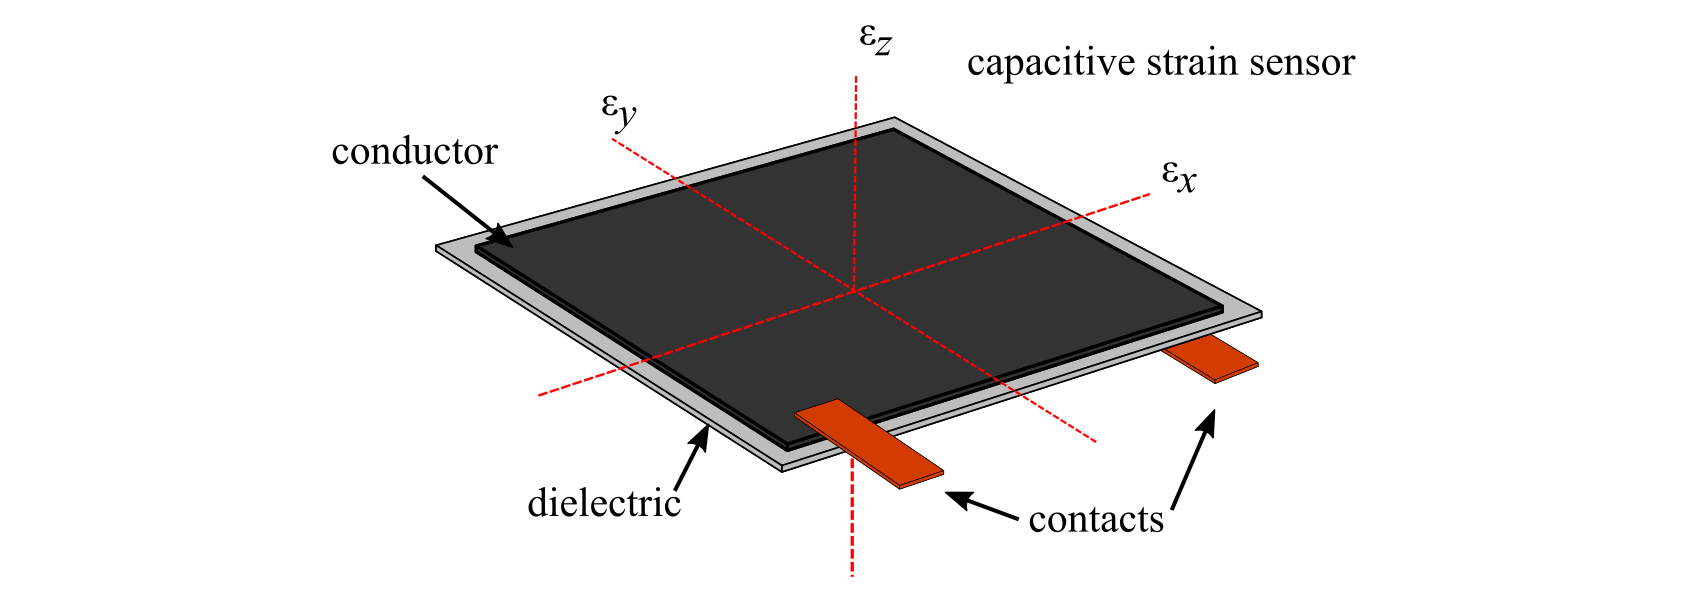
\includegraphics[width=1.0\linewidth]{figures/template_figure.png} \\
\vspace{1\baselineskip} 
\caption{Typical figure example, force the figure to the bottom of a page with [b], or to the top of a page with [t].}
\label{fig:example}
\vspace{2\baselineskip} % A figure needs two to six blank lines to text.)
\end{figure}

A few more lines of text. \lipsum[5]

\FloatBarrier

\bibliographystyle{unsrt}

{\footnotesize\bibliography{IWSHM_template}} % 10 pt font

\end{document}















